\documentclass[openany, longbibliography,slovene,a4paper,12pt]{article}
%\documentclass[openany,slovene,a4paper,12pt]{article}
\usepackage[a4paper,inner=3.5cm,outer=2.5cm,top=2.5cm,bottom=2.5cm]{geometry}

\usepackage{braket}
\usepackage{float}
\usepackage{afterpage}
\usepackage{graphicx}
\usepackage{amssymb}

\usepackage[tbtags]{amsmath}
\usepackage[T1]{fontenc}
\graphicspath{{./slike/}{../slike_vezikel_z_robom/}{/home/jure/sola/magisterij/uporabljene_slike/}
{../eps_pdf/}}
\DeclareGraphicsExtensions{.eps,.jpeg,.png,.gif,.pdf}
\usepackage[outdir=./slike/]{epstopdf}
\epstopdfsetup{
	suffix=,
}
\usepackage[multidot]{grffile}

% \usepackage[slovene]{babel}      % slovenski delilni vzorci (!)
% \usepackage[english]{babel}
\usepackage[utf8]{inputenc}
\usepackage{makeidx}
\usepackage{enumerate}
\usepackage{caption}
\usepackage{subcaption}
\usepackage[tbtags]{mathtools}

\usepackage[section]{placeins}

\usepackage[hyphens,spaces,obeyspaces]{url}
\usepackage{breakurl}


\usepackage{ragged2e}
\edef\UrlBreaks{\do\-\UrlBreaks}

\usepackage{makeidx}
\pagestyle{headings}
\makeindex
\usepackage{fancyhdr}
\usepackage[titletoc,title]{appendix}


\usepackage[sort, numbers]{natbib}
\usepackage[pdfa]{hyperref}
\usepackage[x-1a]{pdfx}
\usepackage{pdfpages}
\usepackage{breqn}


\DeclareMathOperator{\arcsinh}{arcsinh}

\def\epsfg#1#2{\epsfig{file=#1.eps,width=#2}}
\def\legendamp#1#2{\vbox{\hsize=#1\caption{\small #2}}}

\setcounter{topnumber}{4}
\setcounter{bottomnumber}{4}
\setcounter{totalnumber}{5}
\renewcommand{\topfraction}{0.99}
\renewcommand{\bottomfraction}{0.99}
\renewcommand{\textfraction}{0.0}
\setlength{\tabcolsep}{10pt}
\renewcommand{\arraystretch}{1.5}

\def\bi#1{\hbox{\boldmath{$#1$}}}
\let\oldvec\vec
\def\vec#1{\mbox{\boldmath$#1$}}
\def\pol{{\textstyle{1\over2}}}
\def\svec#1{\mbox{{\scriptsize \boldmath$#1$}}}

\newcommand{\dif}{\mathrm{d}}
\usepackage{xparse}
\DeclareDocumentCommand{\myint}{o m o o}  
{%
	\int \IfValueT{#1}{#1} \dif #2 \IfValueT{#3}{\dif#3} \IfValueT{#4}{\dif#4}
}
\newcommand{\Alpha}{A}
\newcommand{\Beta}{B}
\newcommand{\Epsilon}{E}
\newcommand{\Kappa}{K}


\begin{document}
\section{Introduction}
One of the most important basic problems in physics is the dynamics of many-body
systems. Specificaly, in quantum physics and chemistry, the dynamics of
electrons and their spatial distribution determine the stability of matter. But
it is not just the stability that matters. Electronic structure of materials
determines many macroscopic properties like thermal and electrical conductivity, their response to electronic and magnetic fields, etc.

Calculation of electronic structure has always been a challenge. It quickly
became apparent that direct use of Schr{\"o}dinger equation is not a realistic
prospect for calculation of electronic structure, except for some small
molecules, as the time consumed to solve it grows exponentially
\cite{nobel_lecture} as a function of electron
number. With the development of computers different numerical approximations for
computation of electronic structure and optimization of molecular structure have
emerged. One of the most successful methods has been density functional theory
(DFT from now on), which has been known for roughly 50 years. Through the years DFT has developed and today it represents one of the main tools for calculation of electronic structure especially for complex molecules and crystals.

\section{Hamilotnian}
The first step in formulation of the problem is to define hamiltonian which
describes motion of nuclei and electrons. Non-relativistic hamiltonian
describing the interaction of  nuclei and electrons can be written as follows:
\begin{equation} \label{full_hamiltonian}
\hat H= \hat T_n + \hat  T_e + \hat  W_{n-n} + \hat W_{e-e} + \hat W_{n-e} + \hat V_{ext},
\end{equation}
where $T_n$ and $T_e$ are kinetic energies of nuclei and electrons respectively,
$W_{n-n}$, $W_{e-e}$ and $W_{e-n}$ represent  nuclei-nuclei, electron-electron
and electron-nuclei interaction terms. $V_{ext}$ is strictly multiplicative external potential. Ground state of such system is given by the solution of time independent Schr{\"o}dinger equation:
\begin{equation} \label{ham_solution}
\hat H \psi = \epsilon_0 \psi_0,
\end{equation} 
where index $0$ denotes the solution with the lowest energy. In general $\psi_0$
depends on $3N$ coordinates, where $N$ is total number of particles. This means
that systems with more than e.g. 10 atoms are very computationally
demanding. It is common to reduce the dimensionality of the problem by employing
Born-Oppenheimer approximation in which the motion of nuclei is separated from
motion of electrons, sometimes even fixed. Thus, from now on we will restrict
ourselves to hamiltonians describing only the motion of electrons:
\begin{equation} \label{electron_hamiltonian}
\hat H=  \hat  T_e  + \hat W_{e-e} + \hat W_{n-e} + \hat V_{ext}.
\end{equation}
The number of electrons $N$ for a small molecules, like water, is of the order $\sim
10$. In medium sized molecules with $\sim 50-100$ atoms, the number can grow to a few
hundred, while in large molecules, like proteins, the number can grow into
thousands and ten-thousands. As one can imagine, solving a system of coupled differential equations
with such huge number of coordinates ($3N$) is computationally very intensive
procedure and not suitable for mass research usage.
This is the reason for development of approaches which, while still being
sufficiently accurate, offer faster computational times. DFT represents one of
the most successful methods to solving such systems.

\section{Density functional theory - DFT}
DFT is a method, which allows us to map many-particle problem to an effectively
single particle problem. It replaces all electron wave function with
particle density.  The core of DFT lies in Kohn-Sham theorems. These two theorems
ensure that stationary many-particle systems are fully characterized by their
ground state particle density. For non-degenerate case the latter is uniquely determined
by ground state many-particle wave function, which in turn is uniquely determined by the
external potential. For a simple non-degenerate case we will prove this theorem.
Let us consider hamiltonian of the form:
\begin{equation} \label{ks_hamiltonian}
\hat H = \hat T + \hat W + \hat V_{ext},
\end{equation}
where $T$ is kinetic energy, $W$ is inter-particle interaction and $V$ is external
potential determined up to a constant. Let $V_{ext}$ be such potential that
ground state $\psi_0$ is non-degenerate. Consider now the set of all $H$ of the
form (\ref{ks_hamiltonian}), which differ only in $V_{ext}$, with non-degenerate
ground states. Since kinetic and inter-particle interaction terms are the same
for all $H$ in such set, the latter can be represented by the set of all non-equivalent potentials:
\begin{equation}
  \begin{split}
    \mathcal{V} = \{V_{ext};\quad &\textrm{V determined up to multiplication factor and a constant;}\\
    & \textrm{$\ket{\psi_o}$ is exists and is non-degenerate}\}
    \end{split}
 \end{equation}
According to the above definition we can define the set of all corresponding
ground state-densities determined up to phase as:
\begin{equation}
  \begin{split}
    \mathcal{G} = \{\psi_0; \quad &\textrm{$\psi_0$ ground state corresponding to a potential from $V$;}\\
&\textrm{ $\psi_0\sim\psi_0e^{i\phi}$   }
    \}
    \end{split}
  \end{equation}
The map from $\mathcal{V}$ to $\mathcal{G}$ is surjective by definition. What we
would like to know is, if it is also injective  (\ref{bijection}), i.e., can a single $\psi_0$ be a
ground state for two non-equivalent potentials? Suppose now that $\psi_0$ is a
ground state for two non-equivalent potentials $V_{ext}$ and $V'_{ext}$.

\begin{figure}
  \centering
  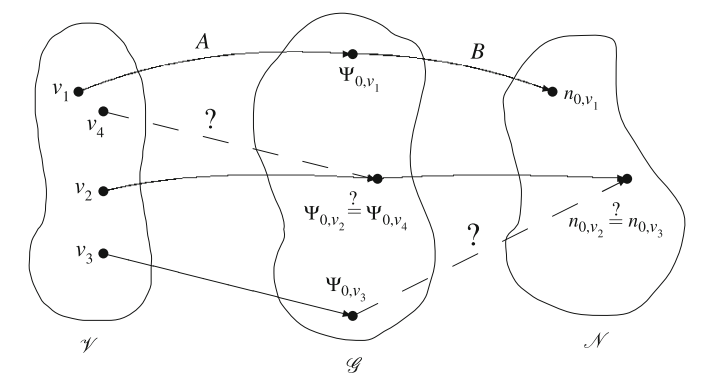
\includegraphics[width=0.55\textwidth]{bijekcija_med_v_psi_n.png}.
  \caption{Bijection between the set of potentials, their corresponding ground
    states and ground state densities. Existance of such bijection is proven by
    Kohn-Sham theorems and proves that multi-particle system is
    uniquely determined by it's ground state particle
    density~\cite{advanced_course}.}
  \label{bijection}
\end{figure}

\begin{dgroup*}
\begin{dmath}
 \hat H\ket{\psi_0} =(\hat T + \hat W + \hat V_{ext}) \ket{\psi_0}\hiderel{=}\epsilon_0\ket{\psi_0}
\end{dmath},
\begin{dmath}
 \hat H'\ket{\psi_0} =(\hat T + \hat W + \hat V'_{ext}) \ket{\psi_0}\hiderel{=}\epsilon'_0\ket{\psi_0}
\end{dmath},
\begin{dsuspend}
subtracting above equation yields:
\end{dsuspend}
\begin{dmath}
(\hat V_{ext} - \hat V'_{ext})\ket{\psi_0}=(\epsilon_0-\epsilon'_0)\ket{\psi_0}
\end{dmath}.
\begin{dsuspend}
 due to multiplicative nature of potentials, we can just divide the whole
 equation by $\ket{\psi_0}$ and obtain: 
\end{dsuspend}
\begin{dmath}
  (\hat V_{ext} - \hat V'_{ext})=(\epsilon_0-\epsilon'_0),
  \end{dmath}
\end{dgroup*}
which is contradiction, since must $V_{ext}$ and $V'_{ext}$ differ for more than a
constant. Similarly one can show that two different grounds state wave functions,
corresponding to two different external potentials, cannot lead to the same
ground state densities.  To see this we compare ground state energies and rewrite
them using ground state densities, which is supposed to be the same for both
wave functions:

\begin{dgroup*}
\begin{dmath}
 \bra{\psi_o}\hat H\ket{\psi_0}=\epsilon_0 < \bra{\psi'_o}\hat H\ket{\psi'_0}=
 \bra{\psi'_o}\hat H + \hat V'_{ext} - \hat V'_{ext} \ket{\psi'_0}=\\ \epsilon'_0
 +  \bra{\psi'_o} \hat V_{ext} - \hat V'_{ext} \ket{\psi'_0}.
\end{dmath}
\begin{dsuspend}
 Rewriting this in terms of densities and taking into account equivalence of H
 and H' yields:
\end{dsuspend}
\begin{dmath}
\epsilon_0 <  \epsilon'_0 + \int (V_{ext}(\vec r)-V'_{ext}(\vec r))n(\vec r)
\dif \vec r ,
\end{dmath}
\begin{dmath}
\epsilon'_0 <  \epsilon_0 + \int (V'_{ext}(\vec r)-V_{ext}(\vec r))n(\vec r)
\dif \vec r.
\end{dmath}
\begin{dsuspend}
  Upon subtracting both equations one obtains a contradiction:
\end{dsuspend}
\begin{dmath}
  \epsilon_0 + \epsilon'_0< \epsilon_0 + \epsilon'_0,
\end{dmath}
\end{dgroup*}
which proves that for hamiltonians which yield non-degenerate ground states,
each ground state leads to a different ground state particle density. Ground
state particle densities form a set where each density corresponds to a single
wave function from $\mathcal G$:
\begin{equation}
  \mathcal N = \left\{n; \bra{\psi}\hat n \ket{\psi}, \psi \in \mathcal G \right\},
\end{equation}
where $\hat n$ is quantum mechanical particle density operator.

Extension of this simple prove to hamiltonians with degenerate ground states is possible
by replacing ground state wave functions by linear span of degenerate ground
states. Thus in degenerate case one obtains bijection between external
potential, set of linear spans, each belonging to a certain external potential
and a set of sets of ground state densities. Special treatment is necessary also
for systems containing magnetic fields, where one can separate hamiltonian into
spin up and spin down hamiltonian of the form (\ref{ks_hamiltonian}). In the
latter case one can obtain bijections between the set of pairs $(\vec A(\vec r),
V_{ext}(\vec r))$, $(\psi_\uparrow, \psi_{\downarrow})$ and $(n(\vec r), \vec m
(\vec r))$.

Since there exists bijection between ground state wave functions and ground
state densities, one can formally rewrite ground state wave function as functional of ground
state particle density:
\begin{equation}
  \ket{\psi'_0} =  \ket{\psi'_0[n]}
  \end{equation}
and using above formula one can also rewrite operators in terms of ground state
density. As an example, let us rewrite ground state energy as functional of
ground state particle density:
\begin{equation} \label{hamiltonian_density}
  E[n_0] = \bra{\psi_0[n_0]}\hat H \ket{\psi_0[n_0]}.
  \end{equation}

for which one can find minimum energy principle: $E[n_0]<E[n]$ whenever n
belongs to $\mathcal N$. This an obvious consequence of wave function functional
$\ket{\psi [n]}$, which is only defined for densities which are in $\mathcal N$.
Thus, one has to ask himself whether every nonegative normalizable function
$n(\vec r)$ is in $\mathcal N$.  The answer is no. A density from $\mathcal N$
have a corresponding potential $V_{ext}$ such that it minimizes energy functional
of the form \ref{hamiltonian_density} and consequently they are called V-representable densities. 

In practice, one does not need deep knowledge about such mathematical
definitions of functionals. The reason for this is the discretization of space into
grid points. On final grid for any strictly positive particle density ($n(\vec r) > 0$),
which is compatible with Pauli principle, there exists a  potential for which the
density represents ground state density and is thus contained in $\mathcal N$ \cite{advanced_course}.

The set $\mathcal N$ is not know and to ensure the problem is also
mathematically well defined, one has to make a transition from
v-representability to N-representability. Let us first redefine our problem in
the form of Levy-Lieb functional:
\begin{dgroup*}
\begin{dmath}
E_{LL}[n]=F_{LL}[n] + \int V_{ext}(\vec r)n(\vec r)
\end{dmath}
\begin{dmath}
F_{LL}=\inf_{\psi \rightarrow n }\bra{\psi} \hat T + \hat W \ket{\psi},
\end{dmath}
\end{dgroup*}
where $\psi \rightarrow n$ means that infimum has to be taken over all
N-particle wave functions, i.e. over all N-representable densities. Levy-Lieb
functional is an extension of Kohn-Sham energy functional and it has a
minimum for exactly the same electron density $n(\vec r)$ \cite{advanced_course}:
\begin{dgroup*}
\begin{dmath}
E_{0}= \min_{n}\left( \inf_{\psi \rightarrow n}\bra{\psi} \hat H +  \hat W +
  V_{ext} \ket{\psi}  \right) = E_{LL}[N].
\end{dmath}
\end{dgroup*}
The set of v-representable densities is a subset of  N-representable densities,
since not all N-electron wave functions necessarily represent ground state for some
external potential $V_{ext}$ \cite{Density-functional_theory_of_atoms_and_molecules}.

The next very important result is that one can construct $N$-electron anti-symmetric wave function
from every non-negative, normalizable function $ n(\vec r)$
\cite{Density-functional_theory_of_atoms_and_molecules, advanced_course}. Thus, Levy-Lieb
functional is, in principle, well defined for any non-negative, normalizable
function $n(\vec r)$.

To construct an anti-symmetric N-electron wave function one can use the
following procedure \cite{Density-functional_theory_of_atoms_and_molecules, advanced_course}:

\begin{dgroup*}
\begin{dmath} \label{phi_k}
\Phi_k(\vec r) = \sqrt { \frac{n(\vec r)}{N}} e^{i \left [\vec k \cdot \vec f (\vec r) + \phi
  (\vec r)\right]}; \quad  k \hiderel \in \mathbb{Z}, 
\end{dmath}
\begin{dsuspend}
  where $\phi(\vec r)$ is an arbitrary scalar function and $f(\vec r)$ is a
  vector field given by:
\end{dsuspend}
\begin{dmath}
  f_x(\vec r) = 2\pi \frac{ \int_{-\infty}^{x}\dif x' n(x', y,z)  } {
    \int_{-\infty}^{\infty} \dif x' n(x', y,z)    }
\end{dmath}
\begin{dmath}
  f_x(\vec r) = 2\pi \frac{ \int_{-\infty}^{\infty} \dif x'
    \int_{-\infty}^{y}\dif y' n(x', y',z)  } {
    \int_{-\infty}^{\infty} \dif x'  \int_{-\infty}^{\infty} \dif y' n(x', y' ,z)    }
\end{dmath}
\begin{dmath}
  f_x(\vec r) = 2\pi \frac{ \int_{-\infty}^{\infty} \dif x'  \int_{-\infty}^{\infty}
    \dif y'
     \int_{-\infty}^{z} \dif z' n(x', y',z')  } {
    \int_{-\infty}^{\infty} \dif x'  \int_{-\infty}^{\infty}
    \dif y'
     \int_{-\infty}^{\infty} \dif z' n(x', y', z')   }.
 \end{dmath}
 \begin{dsuspend}
Using Slater determinan one can  now construct  $N$-particle wave function from
$\phi_k({\vec r})$:
\end{dsuspend}
\begin{dmath}\label{slater_determinant}
  \Phi ({\vec r}) = \frac{1}{\sqrt{N}} \det \left(  \phi_1
    \phi_2 ...  \phi_N  \right).
  \end{dmath}
\end{dgroup*}

Above discussion tells us that minimization principle indeed holds for all
non-negative, normalizable densities, but it says nothing about definitness of
functional. For a given functional to be even defined for given particle
density, the following has to hold separately \cite{advanced_course}:
\begin{dgroup*}
  \begin{dmath} \label{kinetic_inequality}
    \bra{\psi}\hat T \ket{\psi} < \infty
    \end{dmath}
  \begin{dmath} \label{interaction_inequality}
    \bra{\psi}\hat W \ket{\psi} < \infty
  \end{dmath}
    \begin{dmath} \label{potential_inequality}
    \bra{\psi}\hat V \ket{\psi} < \infty.
    \end{dmath}
  \end{dgroup*}
  After deeper mathematical analysis of above equations, on can deduce that both
  $\psi$ and $n^{1/2}$ have to be from Sobolev space defined by:
  \begin{equation}
    \mathcal H = \left\{  f; f \in \mathcal L ^2 \textrm{ and  } \nabla f \in \mathcal{L}^2  \right\},
    \end{equation}
  where $\mathcal{L}$ is a space of functions with finite second norm. The of
  N-representable densities is now known exactly:
  \begin{equation}
    \mathcal{N} = \left\{  n; \int n(\vec r)\dif \vec r=N;    n \in \mathcal H \textrm{ and  } 0  \leq n(\vec r)  \right\},
  \end{equation}
  
  Equations \ref{kinetic_inequality} and \ref{interaction_inequality} have
  imposed restrictions on permissible wavefunctions and densities. Equation
  \ref{potential_inequality} also imposes restriction on potentials. They should
  be of the form $\mathcal{L}^{3/2}+ \mathcal{L}^{\infty}$, thus every potential
  should consist of a part with a finite $\infty$-norm and a part with a
  finite ${3/2}$-norm. As it turns out, the coluomb potential satisfies all
  requirements.

  Above restrictions narrow the possible choices for density function to be used
  in Levy-Lieb functional. Unfortunately, although the domain of Levy-Lieb
  functional has now become well defined it is still not suitable for practical
  use.
  A very serious drawback is that the functional is not convex and may lead to several
  non-minimum stationary points \cite{deriv_lieb_defin_energ_funct} whereas
  Convex functionals have only stationary points which represent local minima.
  Furthermore, convex functionals are naturally differentiable. Fortunately Lieb has
  constructed an alternative functional, which is convex and operates on the
  same domain as Levy Lieb functional (densities and wave functions from sobolev
  space). To define Lieb functional let's first define general energy functional: 
  \begin{equation}
    E[v] = \inf_{\psi}\left\{   \bra{ \psi } H_v \ket{ \psi }  \right\};
    \quad \psi \in \mathcal {H}
    \quad \mathrm{and}
    \quad ||\psi||_2=1.
  \end{equation}
  
  Using this energy functional the Lieb functional is then defined as:
  \begin{equation}
    F_{L}[n] = \sup_{v} \left(  E[v] - \int n(\vec r) v(\vec r) \dif \vec r \right).
  \end{equation}
  Of course $F_{L}[n]$ is again defined only for v-reprezentable densities,
  since calcualtion of $E[v]$ demands conversion $n \rightarrow \psi$. At the
  first glance, it seems that we are back to the original Kohn-Sham functional
  domain. Fortunately, it turn out that the domain of this functional can be
  extended to densities $n(\vec r)$ for which $n^{1/2}(\vec r)$ belongs to
  Sobolev space. The energy is then obtained by:
  \begin{equation} \label{Lieb_energy_v}
    E[v]=\inf_n \left( F_L[n] + \int n(\vec r)v(\vec r)\dif \vec r   \right).
  \end{equation}
  
By extended we mean that it has the same value for every potential belonging to
$\mathcal{L}^{\infty}+ \mathcal{L}^{3/2} $. The proof can be found in \cite{advanced_course}.

  
\subsection{Variational formualtion}
Equation \ref{Lieb_energy_v} defines an extremal problem. To solve it, we have to
find minimium of the functional $E[n]$:
\begin{equation} \label{Lieb_energy_n}
 E[n(\vec r)] =  F_L[n(\vec r)] + \int n(\vec r)v(\vec r)\dif \vec r 
  \end{equation}
 with respect to $n(\vec r)$ and at the same time fulfill predefined particle
 number requirement:
\begin{equation} \label{extremal_problem}
  \frac{\delta }{\delta n(\vec r)} \left[  E[n(\vec r)] - \mu \left(  \int n(\vec r) -N \right)  \right] =0.
\end{equation}
Substituting \ref{Lieb_energy_n} into \ref{extremal_problem} yields
(Euler-Lagrange equations):
\begin{equation} \label{Lieb_derivative}
  \frac{\delta F_L[n(\vec r)]}{\delta n(\vec r)} = -v(\vec r) + \mu.
  \end{equation}
  The functional derivative of Lieb functional is well defined since the
  functional is convex and defined on a dense enough set. Sketch of the proof
  and further references can be found in \cite{advanced_course}. The solution of
  eq. \ref{Lieb_derivative} represent local minima of $E[n]$ and global minimum
  is the same as the one in original N-particle hamiltonian. This result tells
  us that the problem is mathematically well
  defined. Unfortunately, $F_L[n]$ is in general an unknown functional of
  $n(\vec r)$. This prevents us to use this theory unless we find the functional
  $F[n (\vec r)]$ or at least a good approximation. A lot of work has
  been done in this area and there do exist some more or less good approximations,
  depending on the system in question. In the next section we will have a look at dft in a more practical way.

  \section{DFT in practice}
  In the previous section we have had a look at mathematical side of dft and
  it's connection a direct approach of solving N-particle hamiltonian with
  3N coordinates. Now we would like use the knowledge from previous section to
  formulate an approach to solve many electron problem based on Kohn-Sham
  theorems, where particle density has the central role. We will concentrate on
  construction of energy functional $E[n(\vec r)]$, which should approximate
  $F[n(\vec r)]$ as well as possible.
  
  \section{Kohn-Sham equations}
  Kohn-Sham (KS) equations represent a standard and most common approach to dft.
  They are based on energy functional dependent only on electron density $n(\vec
  r)$. To introduce them in an understandable and consistent fashion, let's start with a
  non-interacting system. 
 
\subsection{Noninteracting system}
Hamiltonian of $N$-particle non-interacting system can be written in the
following way:
 \begin{equation} \label{noninteracting_H}
   \hat H =\hat  W_k + \hat V_{ext}, 
 \end{equation}
 where $V_{ext}$ is an external potential of multiplicative nature. It is well
 known the solution to this problem can be written in the form of Slater determinant:

 \[
       \ket{\Phi_0} = \frac{1}{\sqrt{N!}}\det 
   \begin{bmatrix}
   \phi_{1}(\vec r_1, \sigma_1) & \phi_{2}(\vec r_1, \sigma_1) & \phi_{3}(\vec
   r_1, \sigma_1) & \dots & \phi_{N}(\vec r_1, \sigma_1) \\
    \phi_{1}(\vec r_2, \sigma_2) & \phi_{2}(\vec r_2, \sigma_2) & \phi_{3}(\vec
    r_2, \sigma_2) & \dots & \phi_{N}(\vec r_2, \sigma_2) \\
    \vdots & \vdots & \vdots & \ddots & \vdots \\
     \phi_{1}(\vec r_N, \sigma_N) & \phi_{2}(\vec r_N, \sigma_N) & \phi_{3}(\vec r_N, \sigma_N) & \dots & \phi_{N}(\vec r_N, \sigma_N) \\
\end{bmatrix},
\]
 which, when inserted into equation (\ref{noninteracting_H}) effectively produces
 single particle problem:
 \begin{equation}
   \left(-\frac{\hbar^2}{2m}\nabla^2 + \hat V_{ext}(\vec r)\right) \psi (\vec r) = \epsilon_i \psi(\vec r).
 \end{equation}
 Thus, using slater determinant we have effectively converted many particle
 problem with $3N$ coordinates to a single particle problem. Of course the
 particles in this case do not feel each other and motion of each particle
 should not depend on other particles, so such a breakdown is completely natural.
 
 The ground state of such a system is obtained using $N/2$ lowest states by
 putting $2$  electrons into each state. Calculation of kinetic energy and particle
 density for such a system is also straight forward. As we can see, using Slater
 determinant as ansatz for the solution of noninteracting hamiltonian offers
 simple expressions for ground state wavefunction, kinetic energy and particle density
 calculation. Particle density corresponding to such wave function can be written
 using the following expression:
 \begin{equation} \label{KS_density}
   n_0(\vec r) = \sum_{\sigma=\uparrow,\downarrow}\sum_i\Theta(\epsilon_F-\epsilon_i)|\phi_i(\vec r, \sigma)|^2.
 \end{equation}
 The density of electrons is just a sum over all occupied orbitals. Now let's
 remember Kohn-Sham theorems, which state that ground state density is unique
 functional of ground state wave function:
 \begin{equation}
   \ket{\psi}= \ket{\psi(n(\vec r))}.
 \end{equation}
 One can show that there exists an even stronger connection; every $\phi_i$ is a
 uniquely determined by ground state density. One can see this by considering a single
 particle problem using the same potential $V_{ext}$ as found in eq.
 (\ref{noninteracting_H}) and then gradually adding particles, thus:
 \begin{equation}
   \ket{\phi_i}= \ket{\phi_i(n(\vec r))}.
 \end{equation}
 Using this relations we can define HK functional:
 \begin{equation}
   E_s[n(\vec r)] = \bra{\psi[n(\vec r)]}T \ket{\psi(n(\vec r))} + \int \dif \vec r n(\vec r) V_{ext}(\vec r),
   \end{equation}
 where
\begin{equation} \label{KS_kinetic_term}
   T[n(\vec r)] = \sum_i\Theta(\epsilon_F-\epsilon_i)  \sum_{\sigma=\uparrow,\downarrow}\int \phi^*_\sigma(\vec r)\frac{-i\hbar\nabla^2}{2m}\phi_\sigma(\vec r),
 \end{equation}
 where we have implicitly used $\ket{\phi_i(\vec r)} = \ket{ \phi[n(\vec r)] }$.
 In practice this in not necessary, since functions $\phi(\vec r)$ are known -
 they are direct result of calulation.
 
Now we would like to use a similar construction to solve hamiltonian
\ref{hamiltonian_density}. Using solution ansatz in the form of Slater
determinant or some other sum of basis functions (commonly called orbitals) offers straight forward
calculation of kinetic energy and  particle density. Using Slater determinant leads to
differential equations for $\phi_k$ wavefunctions. Modern computational packages
instead of solving differential equations usually use
large sets of basis functions, which in the end lead to over determined set of
algebraic equations. Solution is then given by populating lowest energy orbitals until all electrons
are allocated.
 

First we have to ask ourselves if it is at all possible to convert interacting
$N$ particle problem ($3N$ coordinates) to an effectively single particle (3 coordinates)
problem. By this we mean if there exists a noninteracting system that has the
same groud state electron density as original interacting system.
To see how this is possible consider a $N$ particle interacting system
with $n(\vec r)$ ground state particle density. Since it represents ground
state,  this particle density belongs to $\mathcal H$. Further, using equation
(\ref{slater_determinant}) one can construct non-interacting many particle wave
function, which minimizes hamiltonian of the form (\ref{noninteracting_H})
for some potential $V_{ext}$. Such a system is called Kohn-Sham system/equations.
Thus, we see that there exists a non-interacting system with exactly the same
ground state particle density as originally considered interacting system. The
question still remains what kind of potential should one use in place of many
particle interaction operators still remains open.

Intuitively, one would expect that potential belonging to effective single
particle hamiltonian should reflect the properties, geometry and potentials found
in given many particle system. Hamiltonian naturally contains kinetic energy
term, but it should also somehow contain inter particle interactions. Usually
Kohn-Sham hamiltonian consists of kinetic energy term, Hartree inter particle
interaction, external potential and exchange-correlation functional \cite{advanced_course}:
\begin{equation} \label{KS_system}
  E[n(\vec r)]=T[n(\vec r)]] + E_H[n(\vec r)]] + E_{ext}[n(\vec r)]] + E_{xc}[n(\vec r)]].
\end{equation}
Hartree term is just Coulomb repulsion:
\begin{equation} \label{hartree_term1}
  E_H[n(\vec r)] = \int n(\vec r)w(\vec r, \vec r') n(\vec r')\dif \vec r' \dif \vec r
\end{equation}
including self-repulsion. It is better to calculate Coulomb term using KS wave functions:

\begin{equation} \label{hartree_term2}
   E_H[n(\vec r)] =  \sum_i\Theta(\epsilon_F-\epsilon_i)  \sum_{\sigma=\uparrow,\downarrow}\int \phi^*_\sigma(\vec r')w(\vec r, \vec r')\phi_\sigma(\vec r).
  \end{equation}
Computational packages often employ different approximation and optimizations
for faster calculation of this term \cite{orca}. Functional belonging to
external potential is well known:
\begin{equation} \label{ext_potential_functional}
  E_{ext}[n(\vec r)] = \int n(\vec r) V_{ext}(\vec r) \dif \vec r.
\end{equation}
Unfortunately exchange-correlation functional is much less well known. It is
defined by the equation (\ref{KS_system}) and contains all inter-particle
interactions not contained in $T[n(\vec r)]$. Hartree (\ref{hartree_term2}) and external potential
energy functionals (\ref{ext_potential_functional}) are exact functionals, e.g.
if $\phi_i(\vec r)$ are exact wave functions of electrons in a given system,
then these two functional will produce correct Coulomb repulsion energy and
correct energy of particles in external potential.  The same can not be said for
kinetic energy functional. The difference between exact kinetic energy
of interacting system and $T[n(\vec r)]$ is the exchange energy we are looking for:
\begin{equation}
  E_{xc}^{\psi_0}-E_{xc}[n(\vec r)] = \bra{\psi_0}\hat T \ket{\psi_0} - \bra{\Phi_0}\hat T \ket{\Phi_0},
\end{equation}
where $\ket{\psi_0}$ is the true ground state of interacting system. $\ket
\psi_0$ and $\ket \Phi_0$ may yield completely different electronic states,
but the aim here is to find such $\ket{\Phi_0}$ that both functions yield the
same electron density. *check page 62 and add here*

Our goal is to minimize hamiltonian of the form (\ref{KS_system}) using Slater
determinant as ansatz for many electron system and density calculation. By
considering (\ref{ext_potential_functional}) and (\ref{KS_kinetic_term}) one can
write KS equation:  
\begin{equation}
  \left( \hat T + v_{ext} + E_H[n(\vec r)]]  + E_{xc}[n(\vec r)]] \right) \ket \phi_i =  \epsilon_i \phi_i,  
\end {equation}
where density $n(\vec r)$  has to be calculated according to equation
(\ref{KS_density}). The functions $\phi_i$ are produced by directly solving
differential equation. They are usually determined by inserting ansatz in the
form of gaussian basis functions from which one can
then construct correct single particle states. Multiplying equation by $\bra
\phi_j$ from the left side yields generalized eigenvalue problem:
\begin{equation}
  \bra {\phi_j} \left( \hat T + v_{ext}(\vec r) + E_H[n(\vec r)]]  + E_{xc}[n(\vec r)]] \right) \ket{\phi_i} =  \epsilon_i \braket{ \phi_j |\phi_i }.
\end {equation}

System obviously has to be solved in a self consistent fashion
\ref{self_consistent_scheme}. One starts with the positioning of nuclei into
desired positions and construction of nuclei potentials.In parallel with the
last step starting electron orbitals $\phi^0_i$ are be constructed. Usually they are written
as a series of Gaussian functions. Electron density $n^0$ can then be quickly
calculated from constructed orbitals. The next step is to
calculate functionals $E_H[n(\vec r)]$ and $E_{xc}[n(\vec r)]$. In the next step
equations are solved. The solution are new orbitals $\phi_i^1$  and from them new density $n^1$ is calculated. The latter is then used to
construct new $E_H[n(\vec r)]$ and $E_{xc}[n(\vec r)]$ which are again used to
solve KS equation from which one gets new orbitals $\phi^3$. The procedure is
repeated until the change in density or energy is not small enough. 


\begin{figure}
  \centering
  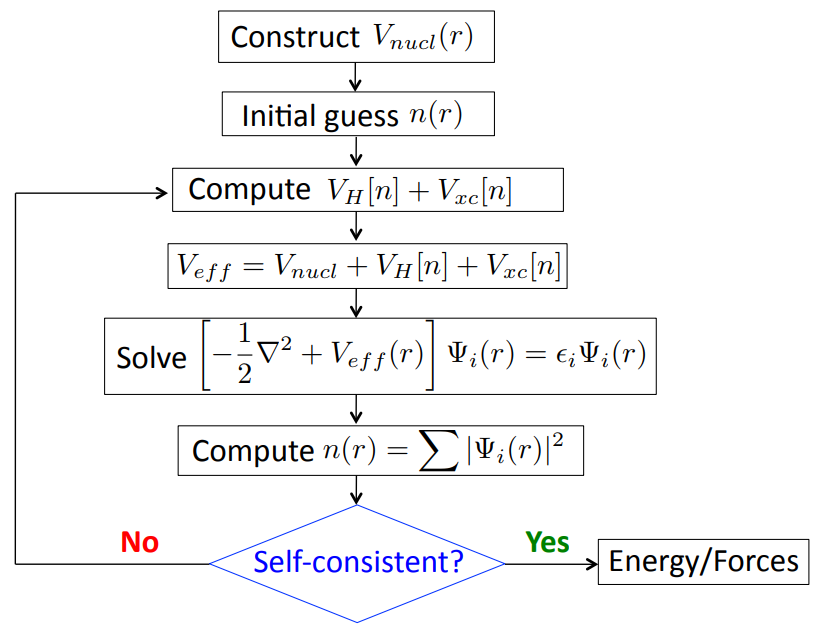
\includegraphics[width=0.65\textwidth]{self_consistent_scheme.png}.
  \caption{Self consistent scheme depicting the procedure in which Kohn Sham
    equations are solved. One starts positioning nuclei into
    desired positions. The next step is to construct potential of nuclei and in
    parallel one can also construct starting approximation for electronic wave
    function. The latter is then used for constructing all other functionals of
    density. After all functionals have been established one can solve KS
    equations, construct new density and repeat the described procedure until
    the change in density is not small enough.
  }
  \label{self_consistent_scheme}
\end{figure}

When given a certain system functionals $T$, $E_H$ and $V_{ext}$ are precisely
determined. $E_{xc}$ is not. It is thus the determining factor for how well the KS
equations describe our system. We will present various functionals used today in
one of the next chapters.

\subsection{Degenerate ground state}
So far we have talked little about the problem of degeneracy of KS states. In
general degeneracy is not a problem, except at Fermi level. When there are more
KS states than there are electrons, several possible ground states and thus also
particle densities can be constructed. In such cases density matrix arising from
several Slater determinants is constructed:
\begin{equation}
  \hat D = \sum_i d_i\ket{\Phi_i} \bra{\Phi_i}.
  \end{equation}
Density belonging to such ground state is just a weighted sum of densities
corresponding to each Slater determinant $n(\vec r)=\sum_id_in_i(\vec r)$, where
$n_i(\vec r)=\sum_j\phi_{ij}(\vec r)$. Index $i$ runs over all possible
Slater determinants one can construct from given degenerate states and index $j$
runs over all states in each Slater determinant. The sum of coefficients $d_k$
is the trace of density matrix and has to be $1$. The choice of coefficients
$d_k$ is not trivial. They have to be constructed in such a way that the new
particle density does not break degeneracy. When a new degenerate state emerges in
scf procedure (fig. \ref{self_consistent_scheme}), it may significantly affect
particle density and resulting potentials and consequently break or destroy
convergence of the procedure. An example is a boron atom where 2p orbitals are
degenerate. Only the choice of $d_{2p^0}=d_{2p^{-1}}=d_{2p^1}=1/3$ leads to spherically symmetric potential and preservation of degeneracy\cite{advanced_course}.

\subsection{Ionization potential}
In general KS eigen functions and eigenvalues do not carry any value in relation
to the real interacting system. There is, however, an exception. Ionization
potential of a finite KS system (a system where density decays exponentially as
$\vec r \rightarrow \infty$) is the same as the ionization potential of real
interacting system \cite{advanced_course}.
  
\subsection{Exchange and correlation functionals}
Exchange and correlation functionals are functionals which try to account for
exchange and correlation interactions between particles. They can be of a
different forms and in general one can roughly divide them into 4 groups \cite{challenges_den_fun_theor}:

\subsubsection{Lda}
Local density approximation (lda) are functionals which depend only on
density of particles (electrons) \cite{challenges_den_fun_theor}.
First functional of such form dates back into
the year 1930, when the exchange interaction for uniform gas was discovered \cite{challenges_den_fun_theor}:
\begin{equation} \label{electron_gas_exchange}
E_{xc}^{lda}[n]=-\frac{3}{4}\left( \frac{3}{\pi} \right)^{1/3}\int n(\vec r)^{4/3} \dif \vec r.
\end{equation}
Today, there exist multiple other lda exchange functionals, but for most cases
they are not very useful. Their only advantage are fast computational times.
For every other purpose gga and hybrid functionals are much better suited.

\subsubsection{Gga}
Generalized gradient approximation (gga) functionals
depend not only on density of particles but also on its gradient \cite{challenges_den_fun_theor}. Most commonly,
gga functionals are build upon (\ref{electron_gas_exchange}) \cite{challenges_den_fun_theor}:
\begin{equation}
  E_{xc}^{gga}=\int n(\vec r)^{4/3}F(x);\quad x=|\nabla n(\vec r)|/n(\vec r)^{4/3}.
\end{equation}
One of most commonly used gga functional is PBE functional
\cite{challenges_den_fun_theor} \cite{challenges_den_fun_theor}:
\begin{equation}
  E_{xc}^{pbe}=-\int  n(\vec r)^{4/3}\left[ \frac{3}{4}\left(\frac{3}{\pi}\right)^{1/3} + \frac{\mu s}{1+ \mu s^2/\kappa} \right]; \quad s=x/(2(3\pi/2)^{1/3}).
\end{equation}
Gga functionals offer acceptable accuracy at fast computational times and are
most commonly used for approximate calculation, before starting more accurate
and more time consuming calcualtion using hybrid or meta-gga functionals.

\subsubsection{Meta-gga functionals}
Since gga functionals have their short commings, meta-gga functionals were formed
in belief that adding higher derivatives will improve accuracy
\cite{challenges_den_fun_theor}. Meta-gga functionals are build upon gga
functional form and add terms containing higher order derivatives of particle
density. Functionals are formulated according to the following equation
\cite{challenges_den_fun_theor}:
\begin{equation}
  E_{xc}^{MGGA}= \int \rho^{4/3}F(\rho(\vec r) \nabla \rho(\vec r), \nabla^2 \rho(\vec r), \tau(\vec r)); \quad \tau=\frac{1}{2}\sum_i |\nabla \phi_i(\vec r)|^2
   \end{equation}

Meta-gga functionals have higher computational cost than gga functionals
Unfortunately, as it turned out, they are not significantly better than gga
functionals and are thus not so popular.

\subsubsection{Hybrid functionals}
On the contrary to meta-gga functionals, hybrid functionals are much more
successful \cite{challenges_den_fun_theor}. These functionals are not a
continuation of lda, gga, meta-gga chain. Instead, they incorporate exact
Hartree-Fock exchange term \cite{challenges_den_fun_theor}:
\begin{equation}
  E^{hf}_{xc}=\sum_ {i,j,\sigma}\int\frac{\phi^*_{i\sigma}(\vec r) \phi_{j\sigma}(\vec r) \phi^*_{j\sigma}(\vec r') \phi_{i\sigma}(\vec r')}{|\vec r - \vec r'|}\dif \vec r \dif \vec r'.
\end{equation}
Such functionals do not break Kohn Sham formalism since the wave functions
$\phi_i(\vec r)$ are unique functional of densities shown in previous chapter.


\begin{figure}
  \centering
  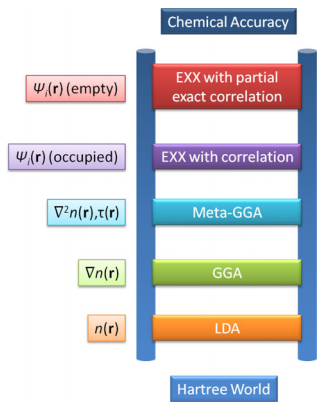
\includegraphics[width=0.45\textwidth]{jacobs_functional_ladder_ver2.png}.
  \caption{Jacob’s ladder of exchange-correlation functional approximations
    employed in dft calculations. Hartree world represents starting level where only
    weak interparticle interaction is present. Lda approxiamtion covers
    functionals which depend only on particle density. Gga additionally depends
    on gradient of particle density, while mega-gga incorporates higher order
    derivatives of particle density and in some cases even kinetic energy of
    orbitals ($\tau$). Hyper-gga functionals, also called hybrid functionals,
    stage represents functionals which contain exact exchange calculation (i.e.
    the one found in Hartree-Fock method). The last level utilizes all Kohn-Sham
    orbitals to calculate correlation and exchange interaction. This level also
    accounts for VdW interaction, which is caused by charge fluctuations and is
    not accounted for in previous stages \cite{How_theo_simul_can_address}.
  }
  \label{bijection}
\end{figure}

\subsection{Van der Waals dispersion}
Dft does not take into account effects caused by charge fluctuations. These Van
der Waals effects can be taken care of with different methods.
The most straight
forward way is simply to add a special non-local functional (VdW-DF method). A similar
approach is to use highly parameterized functionals, like metahybrid
functionals (called DFs). Another way is to add dispersion-corrected
atom-centered potentials (DCACPs). Recently, the most promising seems to be DFT-D method
\cite{consis_accur_ab_initio_param}, which is just a sum of terms $CR^{-6}$
over all atom pairs. As it is generally known, for large distances Van der Waals
potential should decay as $R^{-6}$. It is obvious that DFT-D does obey this
rule as also does VdW-DF method. The other two unfortunately do not obey it. As
a consequence DF and DCACP usually cause underbinding.




\section{All electron dft calculations}
All electron dft calculations are mostly used to calculate electronic structure of
a single molecule. The molecule should not be too big, as otherwise the problem
may become too computationally expensive. Commonly used open source packages
are Orca and Nwchem.

\subsection{Dft using pseudopotentials}
Electronic states of an atom can be divided into three categories; core states,
semi-core states and valence states. The latter are the most actively included
in formation of bonds. Valence states may be completely deformed once the atom
is put into molecules/crystals. Semi-core state are states which do not
directly contribute to bonding, but may still be polarized or spatially
deformed. Lastly, core states, are highly localized and are assumed to be
unaffected by chemical bonding. This means that there should be very little loss
of accuracy if core states are replaced by a pseudo wavefunction.
Pseudo potentials are constructs which try to
replicate effects of core electrons exerted on semi-core, valence electrons and
thus reproduce correct chemical and physical properties (bonding energy, bond
length, electron localization, magnetization,...).

Of course, pseudo potentials have to be constructed prior to a given calculation using
some other much simpler system. As a consequence, there
exists a question of transferability. Is a potential constructed using some
reference molecule usable for another molecule. The exact answer is
not possible. Many times the only way is to try, especially when transition
elements are in question.


\section{Dft in crystals}
Crystals are periodic structures. This fact is also reflected the shape of
electronic  wave functions, which are Bloch states:
\begin{equation}
  \psi_{n, \vec k}(\vec r) = u_{n, \vec k}(\vec r)e^{i\vec k \vec r};\quad \textrm\quad u_{n,\vec k}(\vec r + \vec R) =  u_{n,\vec k}(\vec r),
\end{equation}
where $\vec R$ is a vector is Bravais lattice of a crystal in question.
Functions $u_{n,\vec k}$ depend on potential at each atomic site.
In ideal case, where core potentials are neglected,
wave functions are simple plane waves. When potential is weak and
reasonably smooth, it can be treated as perturbation. Unfortunately neither of
the two conditions is true. Core potential diverges as $r \rightarrow 0$
and as a consequence the wave functions have a cusp at the origin. For heavier
atoms core states have large gradients and can not be represented as plane waves.

The simplest solution is to expand wave functions into series of plane waves.
Computationally this is just a discrete fourier transform of a wave function.
However, because of already given reasons, the number of plane waves required
for such expansion is very large. Thus, even the sum of plane waves is not a
suitable representation of core states. For this reason, core states are
commonly replaced by pseudo potentials in crystal dft calculations. This
approach usually carries \emph{PW calculation} designation.

Although, for many crystals this approach works well it is no good enough
especially for transition elements with partially filled d-shells and second row
elements. Electron density of transition metals and second row elements still
varies widely in spite of use of pseudopotentials. For such cases an improved
approach has been developed. A new method, called gaussian augmented plane waves or \emph{GAPW} approach. GAPW
basis sets consist of Gaussian functions and plane waves. This approach is suitable for all electron
calculations, where core states are expanded in Gaussian functions and valence
electrons in plane waves. As a consequence, all electron wave calculations are
possible for crystals avoiding pseudo potential inaccuracy issues.

\newpage \phantomsection


\addcontentsline{toc}{section}{Literatura}
\bibliographystyle{myapsrevSLO}
\bibliography{mybib}

\end{document}